\subsection{Exercise~2.20}

\begin{proposition}
	\label{equalizers into hausdorff spaces are closed}
	Let~$X$ and~$Y$ be two topological spaces and let~$f$ and~$g$ be two continuous maps from~$X$ to~$Y$.
	Suppose that~$Y$ is a Hausdorff space.
	Then the set~$\{ x ∈ X \suchthat f x = g x \}$ is closed in~$X$.
\end{proposition}

\begin{proof}
	The map
	\[
		φ \colon X \to Y × Y \,, \quad x \mapsto (f x, g x)
	\]
	is continuous by the universal property of the quotient map.
	The diagonal set~$Δ_Y = \{ (y, y) \suchthat y ∈ Y \}$ is closed in~$Y$ because~$Y$ is a Hausdorff space.
	The given set is the preimage~$φ^{-1} Δ_Y$, which is by the continuity of~$φ$ closed in~$X$.
\end{proof}

Suppose first that~$Y$ is a Hausdorff space.
The graph~$Γ$ may be described as
\[
	Γ = \{ z ∈ X × Y \suchthat π_2 z = f π_1 z \}
\]
where~$π_1$ and~$π_2$ are the canonical projections from~$X × Y$ to~$X$ and~$Y$ respectively.
It follows from the above \lcnamecref{equalizers into hausdorff spaces are closed} that~$Γ$ is closed in~$X × Y$.

Suppose now that the graph~$Γ$ is closed in~$X × Y$ and that the space~$Y$ is compact (though not necessarily a Hausdorff space).
Let~$C$ be a closed subset of~$Y$.
The set~$π_2^{-1} C = X × C$ is closed in~$X × Y$, whence the intersection~$Γ ∩ (X × C)$ is again closed in~$X × Y$.
It follows from the compactness of~$Y$ that the projection map~$π_1$ is closed, see Exercise~2.17.
Consequently, the set
\begin{align*}
	π_1 (Γ ∩ (X × C))
	&=
	\{ x ∈ X \suchthat \text{there exists~$y ∈ Y$ with~$(x, y) ∈ Γ ∩ (X × C)$} \} \\
	&=
	\{ x ∈ X \suchthat (x, f x) ∈ X × C \} \\
	&=
	\{ x ∈ X \suchthat f x ∈ C \} \\
	&=
	f^{-1} C
\end{align*}
is closed in~$X$.
This shows that preimages under~$f$ of closed subsets of~$Y$ are closed in~$X$.
Therefore,~$f$ is continuous.

We have used the Hausdorff property for one implication, and compactness for the other implication.

The statement may not hold if~$Y$ is not compact, even if~$X$ and~$Y$ are quite nice.
We may, for example, consider the compact Hausdorff space~$X = [-1, 1]$, the locally compact Hausdorff space~$Y = ℝ$, and the map
\[
	f
	\colon
	X \to Y \,,
	\quad
	x
	\mapsto
	\begin{cases*}
		0   & if~$x ≤ 0$, \\
		1/x & if~$x > 0$.
	\end{cases*}
\]
The graph of~$f$ is closed in~$[-1, 1] × ℝ$, but~$f$ is not continuous.
See \cref{non-continuous function with closed graph} for a picture of the graph of~$f$.
\begin{figure}
	\centering
	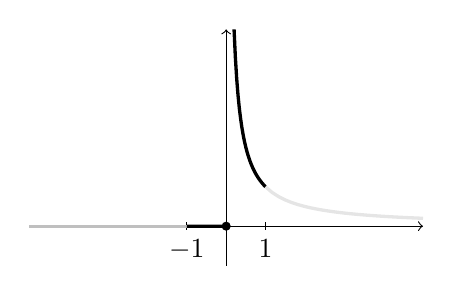
\begin{tikzpicture}[scale = 0.5]
		% axes
		\draw[->] (-5,  0) -- (5, 0);
		\draw[->] ( 0, -1) -- (0, 5);
		\draw (-1, 0.1) -- (-1, -0.1) node[below]{$-1$};
		\draw (1, 0.1) -- (1, -0.1) node[below]{$1$};
		% the line part
		\draw[very thick, gray!50] (-5, 0) -- (-1, 0);
		\draw[very thick, fill] (-1, 0) -- (0,0) circle (0.07);
		% the curver part
		\draw[very thick, domain=0.2:1] plot (\x,{1/\x});
		\draw[very thick, domain=1:5, gray!20] plot (\x,{1/\x});
	\end{tikzpicture}
	\caption{A non-continuous function~$[-1, 1] \to ℝ$ with closed graph.}
	\label{non-continuous function with closed graph}
\end{figure}

This begs the following question:
\begin{quote}
	Let~$Y$ be a topological space such that for every other topological space~$X$, every map~$f \colon X \to Y$ with closed graph is continuous.
	Then must~$Y$ be compact?
\end{quote}
The author doesn’t know the answer to this question.
